\documentclass[
11pt, % The default document font size, options: 10pt, 11pt, 12pt
%codirector, % Uncomment to add a codirector to the title page
]{charter} 




% El títulos de la memoria, se usa en la carátula y se puede usar el cualquier lugar del documento con el comando \ttitle
\titulo{Clasificación de reclamos de usuarios} 

% Nombre del posgrado, se usa en la carátula y se puede usar el cualquier lugar del documento con el comando \degreename
%\posgrado{Carrera de Especialización en Sistemas Embebidos} 
%\posgrado{Carrera de Especialización en Internet de las Cosas} 
\posgrado{Carrera de Especialización en Inteligencia Artificial}
%\posgrado{Maestría en Sistemas Embebidos} 
%\posgrado{Maestría en Internet de las cosas}

% Tu nombre, se puede usar el cualquier lugar del documento con el comando \authorname
\autor{Ing. Lucas Rivela} 

% El nombre del director y co-director, se puede usar el cualquier lugar del documento con el comando \supname y \cosupname y \pertesupname y \pertecosupname
\director{Mg. Lic. Rodrigo Cárdenas}
\pertenenciaDirector{FIUBA} 
% FIXME:NO IMPLEMENTADO EL CODIRECTOR ni su pertenencia
\codirector{John Doe} % para que aparezca en la portada se debe descomentar la opción codirector en el documentclass
\pertenenciaCoDirector{FIUBA}

% Nombre del cliente, quien va a aprobar los resultados del proyecto, se puede usar con el comando \clientename y \empclientename
\cliente{Lic. Nicolás Dagosta}
\empresaCliente{Ualá}

% Nombre y pertenencia de los jurados, se pueden usar el cualquier lugar del documento con el comando \jurunoname, \jurdosname y \jurtresname y \perteunoname, \pertedosname y \pertetresname.
\juradoUno{Nombre y Apellido (1)}
\pertenenciaJurUno{pertenencia (1)} 
\juradoDos{Nombre y Apellido (2)}
\pertenenciaJurDos{pertenencia (2)}
\juradoTres{Nombre y Apellido (3)}
\pertenenciaJurTres{pertenencia (3)}
 
\fechaINICIO{28 de febrero de 2023}		%Fecha de inicio de la cursada de GdP \fechaInicioName
\fechaFINALPlan{24 de abril de 2023} 	%Fecha de final de cursada de GdP
\fechaFINALTrabajo{10 de noviembre de 2023}	%Fecha de defensa pública del trabajo final


\begin{document}

\maketitle
\thispagestyle{empty}
\pagebreak


\thispagestyle{empty}
{\setlength{\parskip}{0pt}
\tableofcontents{}
}
\pagebreak


\section*{Registros de cambios}
\label{sec:registro}


\begin{table}[ht]
\label{tab:registro}
\centering
\begin{tabularx}{\linewidth}{@{}|c|X|c|@{}}
\hline
\rowcolor[HTML]{C0C0C0} 
Revisión & \multicolumn{1}{c|}{\cellcolor[HTML]{C0C0C0}Detalles de los cambios realizados} & Fecha      \\ \hline
0      & Creación del documento                                 &\fechaInicioName \\ \hline
1      & Se completa hasta el punto 5 inclusive                 & 13 de marzo de 2023 \\ \hline
2      & Se completa hasta el punto 9 inclusive                & 20 de marzo de 2023 \\ \hline
%		  Se puede agregar algo más \newline
%		  En distintas líneas \newline
%		  Así                                                    & dd/mm/aaaa \\ \hline
3      & Se completa hasta el punto 12 inclusive                & 27 de marzo de 2023 \\ \hline
%4      & Se completa el plan	                                 & dd/mm/aaaa \\ \hline
\end{tabularx}
\end{table}

\pagebreak



\section*{Acta de constitución del proyecto}
\label{sec:acta}

\begin{flushright}
Buenos Aires, \fechaInicioName
\end{flushright}

\vspace{2cm}

Por medio de la presente se acuerda con el \authorname\hspace{1px} que su Trabajo Final de la \degreename\hspace{1px} se titulará ``\ttitle'', consistirá esencialmente en la implementación de un prototipo de procesamiento de lenguaje natural (PNL)  para la clasificación de reclamos de usuarios, y tendrá un presupuesto preliminar estimado de 600 h de trabajo y U\$D500, con fecha de inicio \fechaInicioName\hspace{1px} y fecha de presentación pública el \fechaFinalName.

Se adjunta a esta acta la planificación inicial.

\vfill

% Esta parte se construye sola con la información que hayan cargado en el preámbulo del documento y no debe modificarla
\begin{table}[ht]
\centering
\begin{tabular}{ccc}
\begin{tabular}[c]{@{}c@{}}Dr. Ing. Ariel Lutenberg \\ Director posgrado FIUBA\end{tabular} & \hspace{2cm} & \begin{tabular}[c]{@{}c@{}}\clientename \\ \empclientename \end{tabular} \vspace{2.5cm} \\ 
\multicolumn{3}{c}{\begin{tabular}[c]{@{}c@{}} \supname \\ Director del Trabajo Final\end{tabular}} \vspace{2.5cm} \\
%\begin{tabular}[c]{@{}c@{}}\jurunoname \\ Jurado del Trabajo Final\end{tabular}     &  & \begin{tabular}[c]{@{}c@{}}\jurdosname\\ Jurado del Trabajo Final\end{tabular}  \vspace{2.5cm}  \\
%\multicolumn{3}{c}{\begin{tabular}[c]{@{}c@{}} \jurtresname\\ Jurado del Trabajo Final\end{tabular}} \vspace{.5cm}                                                                     
\end{tabular}
\end{table}




\section{1. Descripción técnica-conceptual del proyecto a realizar}
\label{sec:descripcion}


%\begin{consigna}{red} % El bloque "consigna" se usa para poner texto en rojo y dar una pequeña ayuda sobre cómo completar la sección. En cada entrega parcial deben eliminar los comandos begin y end del bloque consigna de las secciones que hayan completado.

El objetivo de este proyecto será contar con modelos de inteligencia artificial (IA) que contribuyan a agilizar y mejorar la atención al cliente, mediante la categorización automática de los reclamos de los usuarios. Esto permitirá reducir la cantidad de personas necesarias para la clasificación manual, para que se puedan enfocar en resolver los casos más prioritarios.

Esta propuesta se alinea con la estrategia de la compañía de no tener sucursales abiertas al público, en la cual resulta muy importante que los canales de atención online sean rápidos y efectivos, para así poder asegurarle al cliente una buena calidad de servicio.

En la Figura \ref{fig:figura1} se presenta un diagrama de alto nivel de la solución. Se observa que en primera instancia, los reclamos son recibidos por correo y chat, y luego son registrados en Salesforce.
Diariamente, estos datos son replicados en BigQuery (el Data Warehouse) a través del orquestador Apache Airflow. Estos dos últimos componentes están desplegados en Google Cloud Platform. 

\begin{figure}[H]
\centering 
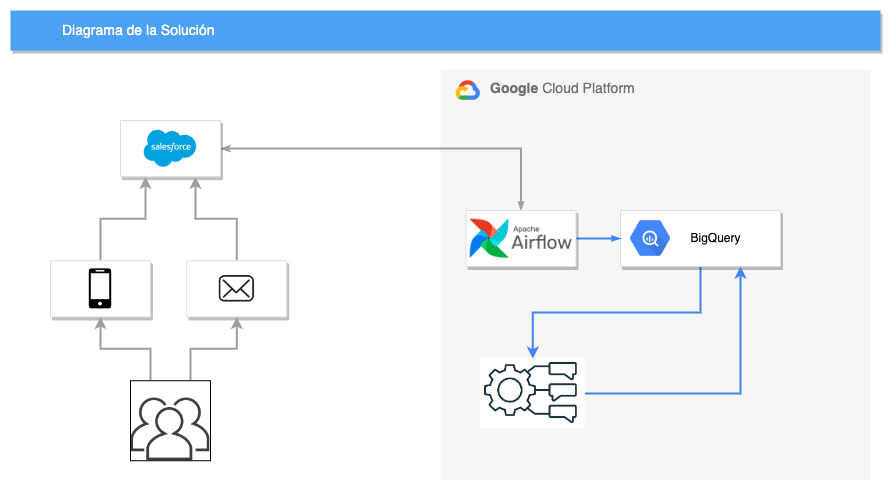
\includegraphics[width=.85\textwidth]{./Figuras/figura1.png}
\caption{Diagrama de alto nivel.}
\label{fig:figura1}
\end{figure}

%\vspace{25px}

Con este proyecto se busca desarrollar y entrenar un modelo clasificador, con los casos de 2021 y 2022 que se encuentran en BigQuery y hayan sido etiquetados manualmente. Una vez desarrollado, se desplegará en la misma nube para realizar las inferencias sobre los nuevos reclamos.

Acerca de la empresa:

Ualá es una \textit{fintech} argentina que brinda su servicio de billetera digital a través de una aplicación móvil. Además, provee una tarjeta prepaga Mastercard para poder operar la cuenta. Los servicios principales que provee son:
\begin{itemize}
	\item Enviar y recibir dinero desde cualquier cuenta bancaria.
	\item Realizar compras nacionales o internacionales con la tarjeta.
	\item Extraer efectivo.
	\item Pagar servicios.
	\item Pedir préstamos o cuotificar consumos.
	\item Realizar ventas a través de \textit{mPOS}, \textit{QR} o link de pago.
	\item Realizar inversiones.
\end{itemize}

%\end{consigna}



\section{2. Identificación y análisis de los interesados}
\label{sec:interesados}




\begin{table}[ht]
%\caption{Identificación de los interesados}
%\label{tab:interesados}
\begin{tabularx}{\linewidth}{@{}|l|X|l|l|@{}}
\hline
\rowcolor[HTML]{C0C0C0} 
Rol           & Nombre y Apellido & Organización 	& Puesto 	\\ \hline
%Auspiciante   &                   &              	&        	\\ \hline
Cliente       & \clientename   & \empclientename	& Gerente de Machine Learning       	\\ \hline
Impulsor      & \clientename   & \empclientename    & Gerente de Machine Learning       	\\ \hline
Responsable   & \authorname       & FIUBA        	& Alumno 	\\ \hline
%Colaboradores &                   &              	&        	\\ \hline
Orientador    & \supname	      & \pertesupname 	& Director Trabajo final \\ \hline
%Equipo        & -                 & -             	& -       	\\ \hline
%Opositores    &                   &              	&        	\\ \hline
Usuario final & Área de atención al cliente        & \empclientename            	& -       	\\ \hline
\end{tabularx}
\end{table}


\begin{itemize}
	\item Impulsor: está interesado en los \textit{insights} que pueda darle este proyecto a nivel tecnológico.
	\item Orientador: cuenta con una gran experiencia en PNL y tiene buena predisposición.
\end{itemize}



\section{3. Propósito del proyecto}
\label{sec:proposito}

%\begin{consigna}{red}
Optimizar el tiempo que lleva el proceso de clasificación de reclamos y consultas mediante su automatización; y por otro lado, reducir la cantidad de personas necesarias para supervisar esta tarea, de manera tal que puedan enfocarse en el proceso de resolución.
%\end{consigna}

\section{4. Alcance del proyecto}
\label{sec:alcance}

%\begin{consigna}{red}
El alcance de este proyecto está orientado a desarrollar un prototipo de solución de software que incluirá las siguientes actividades:

\begin{itemize}
	\item Obtención de los datos: se corresponde con el análisis de las fuentes de datos disponibles y su integración al proceso que se plantea desarrollar.
	\item Análisis exploratorio de los datos: se corresponde con las actividades necesarias para generar nuevos \textit{insights}, que sirvan para guiar el desarrollo de los modelos.
	\item Modelado: se corresponde con la generación de variables a partir de los datos disponibles, que luego serán utilizadas para entrenar los modelos. 
	\item Entrenamiento: se corresponde con la generación de distintos modelos de IA, y su comparación a través de métricas, para encontrar el que mejor se adapte a la problemática de negocio. Estas comparaciones se presentarán en un informe de resultados de los modelos.
	\item Despliegue: se corresponde con el diseño de la infraestructura necesaria para ejecutar los modelos de IA y su despliegue en un entorno de desarrollo (no productivo).
	\item Documentación: se corresponde con los documentos de soporte que explican el proceso de modelado, entrenamiento y despliegue de los modelos.
\end{itemize}

El presente proyecto no incluye:

\begin{itemize}
	\item La adaptación de los modelos a nuevas categorías de reclamos que puedan surgir durante el desarrollo o una vez finalizado el desarrollo. Se utilizarán casos resueltos de 2021 y 2022 y las categorías a considerar serán las que existan hasta ese momento. 
	\item La integración de los modelos y su despliegue con el ambiente productivo.
	\item El soporte de la infraestructura desplegada en el entorno de desarrollo.
\end{itemize}

%\end{consigna}


\section{5. Supuestos del proyecto}
\label{sec:supuestos}

%\begin{consigna}{red}
Para el desarrollo del presente proyecto se supone que:

\begin{itemize}
	\item La empresa mantendrá sus operaciones al menos hasta finalizar el desarrollo.
	\item Se Mantendrá la relación laboral con la empresa al menos hasta finalizar el desarrollo.
	\item El desarrollador asignado a este proyecto no tendrá enfermedades graves que puedan alterar los plazos estipulados para las actividades planteadas.
	\item El área de atención al cliente no realizará cambios en su \textit{CRM} que puedan afectar el proceso de réplica de los casos hacia BigQuery, ni que puedan afectar las categorías sobre las cuales se desarrollan los modelos.
	\item El área de Data de la empresa no cambiará su \textit{Cloud Provider} ni modificará su proceso de réplica hacia BigQuery.
	\item Se tendrá acceso a infraestructura cloud para el entrenamiento y despliegue de los modelos.
	\item Las consultas realizadas al área de atención al cliente se resolverán en plazos razonables.
	
\end{itemize}

%\end{consigna}

\section{6. Requerimientos}
\label{sec:requerimientos}

%\begin{consigna}{red}
\begin{enumerate}
	\item Requerimientos funcionales
		\begin{enumerate}
			\item El sistema debe poder detectar la categoría de un reclamo escrito en lenguaje natural.
			\item El sistema debe poder detectar la categoría de una consulta escrita en lenguaje natural.
			\item El usuario debe poder utilizar los resultados de la clasificación desde una base de datos.
			\item El proceso debe ser capaz de interpretar errores de ortografía.
			\item El proceso debe ser capaz de adaptarse a distinta cantidad de palabras en el mensaje.
			\item La solución debe ejecutarse en forma \textit{batch}, corriendo diariamente y tomando los casos del día anterior.
		\end{enumerate}
	\item Requerimientos no funcionales
		\begin{enumerate}
			\item El sistema debe estar desarrollado en lenguaje Python.
			\item El código debe ser versionado con Git.
			\item La solución debe estar desplegada sobre infraestructura de Google Cloud Platform.
			\item La salida de los modelos debe ser almacenada en BigQuery.
			\item El proceso debe ser ejecutado a través del orquestador Apache Airflow.
		\end{enumerate}
	\item Requerimientos de testing
		\begin{enumerate}
			\item Se deben generar métricas de performance de los modelos con el dataset de entrenamiento y de prueba.
		\end{enumerate}
	\item Requerimientos de documentación
		\begin{enumerate}
			\item Se debe confeccionar un documento con el diseño de la arquitectura de alto nivel.
			\item Se debe confeccionar un documento con el diseño de los modelos de IA.
			\item Se debe confeccionar un documento que especifique los datos que consumen los modelos y su origen.
		\end{enumerate}
\end{enumerate}

%\end{consigna}

\section{7. Historias de usuarios (\textit{Product backlog})}
\label{sec:backlog}

%\begin{consigna}{red}
Roles:
\begin{itemize}
	\item Área de atención al cliente
	\item Área de \textit{Machine Learning}
\end{itemize}

Historias de usuario:

\begin{enumerate}
	\item Como área de atención al cliente quiero clasificar automáticamente los reclamos y consultas para poder brindar una mejor atención a los usuarios.
	\item Como área de atención al cliente quiero que el proceso corra diariamente para poder clasificar los reclamos a día cerrado.
	\item Como área de atención al cliente quiero poder consumir los resultados de la clasificación desde una base de datos para poder integrarlo con el sistema utilizado en el área.
	\item Como área de \textit{Machine Learning} quiero tener documentación que detalle la implementación de la solución para que el proyecto se ajuste a nuestras prácticas de desarrollo.
	\item Como área de \textit{Machine Learning} quiero tener métricas de performance de los modelos para tener una referencia y poder monitorear desvíos en el proceso en el futuro.
	
\end{enumerate}

Criterio para calcular los \textit{story points} de cada historia:

\begin{itemize}
	\item Criterio A: Cantidad de trabajo a realizar
	\item Criterio B: Complejidad del trabajo a realizar
	\item Criterio C: Incertidumbre del trabajo a realizar
\end{itemize}

Pesos para los criterios:

\begin{table}[H]
\begin{tabular}{c c c c}
\hline
\rowcolor[HTML]{C0C0C0} 
Nivel           & Criterio A     & Criterio B 	    & Criterio C 	 \\ \hline
Bajo            & 1              & 1	            & 1              \\ \hline
Medio           & 2              & 3                & 5               \\ \hline
Alto            & 5              & 5        	    & 8 	          \\ \hline
\end{tabular}
\end{table}

Story points:

\begin{table}[H]
\begin{tabular}{c c c c c c}
\hline
\rowcolor[HTML]{C0C0C0} 
Historia           & Criterio A     & Criterio B 	    & Criterio C   & Peso resultante  & Fibonacci	 \\ \hline
1                  & 5              & 5	                & 8            &  18              &  21            \\ \hline
2                  & 2              & 1                 & 1            &  4               &  5            \\ \hline
3                  & 2              & 3        	        & 1 	       &  6               &  8              \\ \hline
4                  & 2              & 1        	        & 1 	       &  4               &  5             \\ \hline
5                  & 2              & 3        	        & 1 	       &  6               &  8              \\ \hline
\end{tabular}
\end{table}

%\end{consigna}

\section{8. Entregables principales del proyecto}
\label{sec:entregables}

%\begin{consigna}{red}

Los entregables del proyecto son:

\begin{itemize}
	\item Plan de proyecto.
	\item Código fuente (queda reservado para \empclientename).
	\item Modelos de inteligencia artificial (queda reservado para \empclientename).
	\item Documento con el diseño de arquitectura de alto nivel.
	\item Documento con el diseño de los modelos de inteligencia artificial.
	\item Documento que especifica los datos que consumen los modelos y su origen.
	\item Documento con las métricas de evaluación de los modelos.
	\item Informe de avance.
	\item Memoria del trabajo.
\end{itemize}

%\end{consigna}

\section{9. Desglose del trabajo en tareas}
\label{sec:wbs}

%\begin{consigna}{red}
Se detallan a continuación todas las actividades que se harán en el proyecto para dar cumplimiento a los requerimientos y su duración estimada:

\begin{enumerate}
	\item Planificación general del proyecto (50 h)
		\begin{enumerate}
			\item Redacción de la descripción técnica-conceptual y propósito. (10 h)
			\item Definición del alcance, requerimientos y entregables. (10 h)
			\item Definición de tiempos y presupuesto. (15 h)
			\item Definición de la gestión de riesgos, calidad y procesos de cierre. (15 h)
		\end{enumerate}
	\item Relevamiento (30 h)
		\begin{enumerate}
			\item Reuniones con el área de atención al cliente. (10 h)
			\item Análisis de las fuentes de datos. (10 h)
			\item Análisis del proceso de clasificación de reclamos y consultas. (10 h)
		\end{enumerate}
	\item Análisis exploratorio de los datos (35 h)
		\begin{enumerate}
			\item Análisis de la distribución de categorías. (10 h) 
			\item Análisis de la longitud de los mensajes. (10 h)
			\item Análisis del procesamiento del texto. (15 h)
		\end{enumerate}
	\item Desarrollo (290 h)
		\begin{enumerate}
			\item Programación de \textit{scripts} para obtener datos de entrada de los modelos. (10 h)
			\item Desarrollo del pipeline de preprocesamiento del texto. (90 h)
				\begin{itemize}
					\item Módulo para remover partes comunes de los mensajes. (15 h)
					\item Módulo para remover palabras redundantes. (15 h)
					\item Módulo para remover símbolos. (10 h)
					\item Módulo para corregir faltas de ortografía. (40 h)
					\item Módulo para armar secuencias. (10 h)
				\end{itemize}
			\item Desarrollo y entrenamiento de \textit{embeddings}. (60 h)
				\begin{itemize}
					\item Investigación herramientas de \textit{embeddings}. (20 h)
					\item Selección de herramienta de \textit{embeddings}. (20 h)
					\item Entrenamiento de \textit{embeddings}. (20 h)
				\end{itemize}
			\item Desarrollo y entrenamiento de modelos. (130 h)
				\begin{itemize}
					\item Investigación de arquitecturas de IA que apliquen al problema. (40 h)
					\item Entrenamiento de modelo baseline. (10 h)
					\item Desarrollo de \textit{scripts} para modelos avanzados. (25 h)
					\item Entrenamiento de modelos avanzados - Parte A. (25 h)
					\item Entrenamiento de modelos avanzados - Parte B. (25 h)
					\item Desarrollo de módulo de escritura de resultados en BigQuery. (5 h)
				\end{itemize}
		\end{enumerate}
	\item Evaluación y pruebas (35 h)
		\begin{enumerate}
			\item Obtención de métricas de los modelos. (30 h)
			\item Selección del mejor modelo. (5 h)
		\end{enumerate}
	\item Despliegue (50 h)
		\begin{enumerate}
			\item Diseño de la arquitectura del \textit{pipeline}. (10 h)
			\item Desarrollo de GitHub Actions. (5 h)
			\item Desarrollo de la imagen de Docker. (20 h)
			\item Desarrollo de DAG (Directed Acyclic Graph) de clasificación. (15 h)
		\end{enumerate}
	\item Documentación (30 h)
		\begin{enumerate}
			\item Elaboración de documento de arquitectura alto nivel. (10 h)
			\item Elaboración de documento con el diseño de los modelos de IA. (10 h)
			\item Elaboración de documento con los datos consumidos. (10 h)
		\end{enumerate}
	\item Cierre del proyecto (80 h)
		\begin{enumerate}
			\item Redacción del informe de avance. (20 h)
			\item Redacción de memoria final. (40 h)
			\item Elaboración de presentación para exposición final. (20 h) 
		\end{enumerate}
\end{enumerate}

Cantidad total de horas: (600 h)

%\end{consigna}

\section{10. Diagrama de Activity On Node}
\label{sec:AoN}

%\begin{consigna}{red}
En la Figura 2 se muestra el diagrama Activity On Node. 

\begin{itemize}
	\item La ruta crítica es resaltada mediante flechas rojas.
	\item Las tareas están expresadas en horas.
	\item A pesar de contar con una sola persona asignada al proyecto, se ejecutan tareas relacionadas en paralelo.
	\item Los colores de las cajas representan las tareas principales del WBS de la sección 9.
\end{itemize}

%La figura \ref{fig:AoN} fue elaborada con el paquete latex tikz y pueden consultar la siguiente referencia \textit{online}:

%\url{https://www.overleaf.com/learn/latex/LaTeX_Graphics_using_TikZ:_A_Tutorial_for_Beginners_(Part_3)\%E2\%80\%94Creating_Flowcharts}

%\end{consigna}

\begin{figure}[H]
\centering 
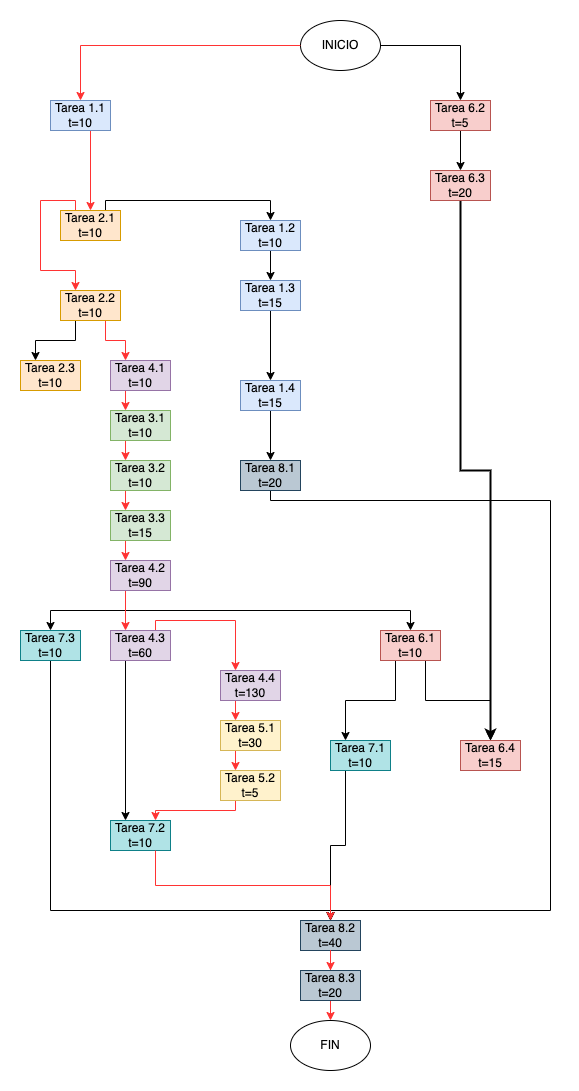
\includegraphics[width=.75\textwidth]{./Figuras/figura2.png}
\caption{Diagrama de \textit{Activity on Node}.}
\label{fig:AoN}
\end{figure}

\begin{landscape}
\section{11. Diagrama de Gantt}
\label{sec:gantt}

%\begin{consigna}{red}
En la figura 3 se muestra el diagrama de Gantt del proyecto.

\begin{figure}[H]
\centering 
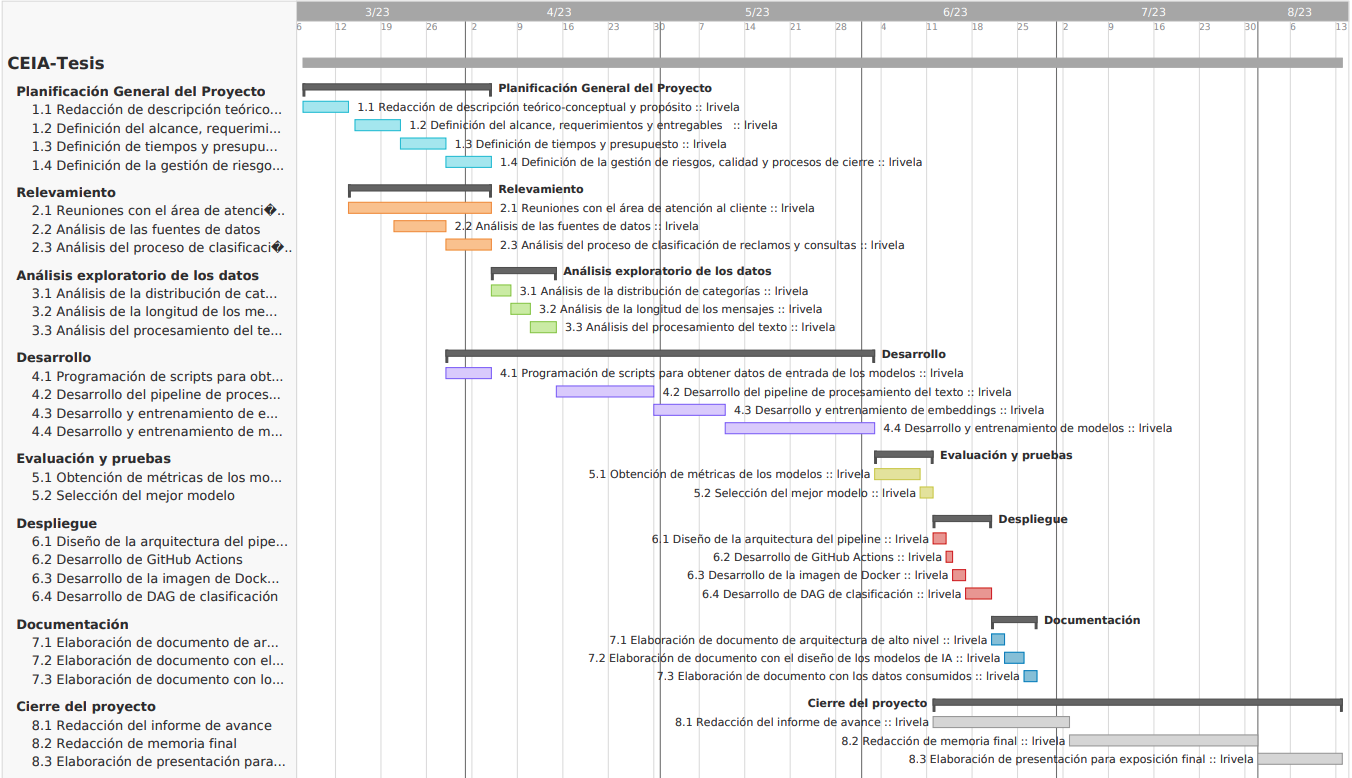
\includegraphics[height=.8\textheight]{./Figuras/figura3.png}
\caption{Diagrama de Gantt}
\label{fig:diagGantt}
\end{figure}
\end{landscape}

%\end{consigna}


\section{12. Presupuesto detallado del proyecto}
\label{sec:presupuesto}

%\begin{consigna}{red}

A continuación, se detalla la composición del presupuesto del proyecto expresado en dólares estadounidenses:

%\end{consigna}

\begin{table}[htpb]
\centering
\begin{tabularx}{\linewidth}{@{}|X|c|r|r|@{}}
\hline
\rowcolor[HTML]{C0C0C0} 
\multicolumn{4}{|c|}{\cellcolor[HTML]{C0C0C0}COSTOS DIRECTOS} \\ \hline
\rowcolor[HTML]{C0C0C0} 
Descripción &
  \multicolumn{1}{c|}{\cellcolor[HTML]{C0C0C0}Cantidad} &
  \multicolumn{1}{c|}{\cellcolor[HTML]{C0C0C0}Valor unitario} &
  \multicolumn{1}{c|}{\cellcolor[HTML]{C0C0C0}Valor total} \\ \hline
Horas de ingeniería &
  \multicolumn{1}{c|}{600 horas} &
  \multicolumn{1}{c|}{\$10 USD} &
  \multicolumn{1}{c|}{\$6000 USD} \\ \hline
Procesamiento en GCP &
  \multicolumn{1}{c|}{200 horas} &
  \multicolumn{1}{c|}{\$1 USD} &
  \multicolumn{1}{c|}{\$200 USD} \\ \hline
Consultas BigQuery & 
  \multicolumn{1}{c|}{1 unidad} &
  \multicolumn{1}{c|}{\$10 USD} &
  \multicolumn{1}{c|}{\$10 USD} \\ \hline
\multicolumn{1}{|l|}{} &
   &
   &
   \\ \hline
\multicolumn{3}{|c|}{SUBTOTAL} &
  \multicolumn{1}{c|}{\$6210 USD} \\ \hline
\rowcolor[HTML]{C0C0C0} 
\multicolumn{4}{|c|}{\cellcolor[HTML]{C0C0C0}COSTOS INDIRECTOS} \\ \hline
\rowcolor[HTML]{C0C0C0} 
Descripción &
  \multicolumn{1}{c|}{\cellcolor[HTML]{C0C0C0}Cantidad} &
  \multicolumn{1}{c|}{\cellcolor[HTML]{C0C0C0}Valor unitario} &
  \multicolumn{1}{c|}{\cellcolor[HTML]{C0C0C0}Valor total} \\ \hline
\multicolumn{1}{|l|}{Notebook} & 1 unidad & \$1200 USD & \$1200 USD \\ \hline
\multicolumn{1}{|l|}{Cloud Storage 20GB} & 1 unidad & \$5 USD & \$5 USD \\ \hline
\multicolumn{1}{|l|}{} &
   &
   &
   \\ \hline
\multicolumn{1}{|l|}{} &
   &
   &
   \\ \hline
\multicolumn{3}{|c|}{SUBTOTAL} &
  \multicolumn{1}{c|}{\$1205 USD} \\ \hline
\rowcolor[HTML]{C0C0C0}
\multicolumn{3}{|c|}{TOTAL} & 
\multicolumn{1}{c|}{\$7415 USD} \\ \hline
\end{tabularx}%
\end{table}


\section{13. Gestión de riesgos}
\label{sec:riesgos}

%\begin{consigna}{red}
Los riesgos asociados al proyecto y sus planes respectivos planes de mitigación son los siguientes:
 
Riesgo 1: no contar con datos distribuidos uniformemente entre las categorías.
\begin{itemize}
	\item Severidad (S): este riesgo tiene una severidad media-alta porque puede influir en la performance final de los modelos de IA. (6)
	\item Probabilidad de ocurrencia (O): la probabilidad de este riesgo es alta porque hay categorías de reclamos que suceden mucho más a menudo que otras. (7)
\end{itemize}   

Riesgo 2: no contar con la infraestructura cloud de la empresa para entrenar los modelos de IA.
\begin{itemize}
	\item Severidad (S): este riesgo tiene una severidad media-alta porque puede alargar las tareas de modelado y entrenamiento. (8)
	\item Ocurrencia (O): la probabilidad de este riesgo es baja porque la utilización de los recursos fue pactada previamente. (4)
\end{itemize}

Riesgo 3: decisión del área de Data de la empresa de cambiar de \textit{Cloud Provider}.
\begin{itemize}
	\item Severidad (S): este riesgo tiene una severidad baja porque no requeriría realizar grandes cambios al utilizar herramientas \textit{open source} para el despliegue. (4)
	\item Ocurrencia (O): la probabilidad de este riesgo es baja porque la adopción de la plataforma es estratégica. (2)
\end{itemize}

Riesgo 4: no poder realizar la clasificación automática con un nivel de precisión aceptable.
\begin{itemize}
	\item Severidad (S): este riesgo tiene una severidad alta porque tener una mala precisión podría hacer que los modelos de IA no se usen. (8)
	\item Ocurrencia (O): la probabilidad de este riesgo es baja porque antes de este proyecto se realizó una prueba piloto para algunas categorías que fueron combinadas y tuvo buenos resultados. (2)
\end{itemize}

Riesgo 5: no contar con herramientas de preprocesamiento de texto en español.
\begin{itemize}
	\item Severidad (S): este riesgo tiene una severidad media-alta porque puede influir en la performance final de los modelos de IA y también porque puede alargar las tareas de preprocesamiento al no poder utilizar herramientas ya desarrolladas. (8)
	\item Ocurrencia (O): la probabilidad de este riesgo es baja ya que se realizó una investigación previa y hay algunas librerías de Python que pueden ser utilizadas para texto en español. (3)
\end{itemize}


b) Tabla de gestión de riesgos: (El RPN se calcula como RPN=SxO)

Criterio adoptado: 
Se tomarán medidas de mitigación en los riesgos cuyos números de RPN sean mayores a 30.

\begin{table}[H]
\centering
\begin{tabular}{@{}|c|c|c|c|c|c|c|@{}}
\hline
\rowcolor[HTML]{C0C0C0} 
Riesgo &  S  &  O  &  RPN  &  S*  &  O*  &  RPN* \\ \hline
   1   &  6  &  7  &  42  &   3   &  7   &  21   \\ \hline
   2   &  8  &  4  &  32  &   6   &  4   &  24   \\ \hline
   3   &  4  &  2  &  8   &   -   &  -   &   -   \\ \hline
   4   &  8  &  2  &  16  &   -   &  -   &   -   \\ \hline
   5   &  8  &  3  &  24  &   -   &  -   &   -   \\ \hline
\end{tabular}%
\end{table}



Nota: los valores marcados con (*) en la tabla corresponden luego de haber aplicado la mitigación.

c) Plan de mitigación de los riesgos que originalmente excedían el RPN máximo establecido:
 
Riesgo 1: se utilizarán técnicas de balanceo de clases.
\begin{itemize}
	\item Severidad (S): la severidad baja considerablemente, ya que al aplicar estas técnicas se intenta disminuir los efectos del desbalanceo en el entrenamiento del modelo. (3)
  	\item Probabilidad de ocurrencia (O): la probabilidad de ocurrencia se mantiene igual. (7)
\end{itemize}

Riesgo 2: se utilizarán alternativas a Google Cloud, como Paperspace, Google Colab o incluso usando hardware físico.
\begin{itemize}
	\item Severidad (S): la severidad baja a un nivel medio, ya que igualmente se podrá entrenar usando placa de video. (6)
  	\item Probabilidad de ocurrencia (O): la probabilidad de ocurrencia se mantiene igual. (4)
\end{itemize}
 

%\end{consigna}


\section{14. Gestión de la calidad}
\label{sec:calidad}

%\begin{consigna}{red}
\begin{itemize} 
	\item Req. \#1.1, Req. \#1.2, Req. \#1.4 y Req. \#1.5: el sistema debe poder detectar la categoría de un reclamo o consulta escrito en lenguaje natural, con o sin errores de ortografía y cantidad de palabras variable.
	\begin{itemize}
		\item Verificación: se probarán mensajes de distintas longitudes, con y sin errores y se revisará que se asigne una categoría.
		\item Validación: se revisarán con el cliente distintos mensajes de entrada y la categoría asignada.
	\end{itemize}
	\item Req. \#1.6: la solución debe ejecutarse en forma \textit{batch}, corriendo diariamente y tomando los casos del día anterior.
	\begin{itemize}
		\item Verificación: se implementará un \textit{cronjob} que refleje una periodicidad diaria, corriendo por la mañana y tomando los casos del día cerrado inmediatamente anterior. 
		\item Validación: se dejará el \textit{schedule} activado y se controlará al día siguiente la ejecución automática con el cliente.
	\end{itemize}
	\item Req. \#2.3: la solución debe estar desplegada sobre infraestructura de Google Cloud Platform.
	\begin{itemize}
		\item Verificación: la solución se implementará usando componentes de infraestructura que hayan sido previamente desplegadas en el área de \textit{Machine Learning}.
		\item Validación: se controlará con el cliente que los componentes elegidos sean los adecuados.
	\end{itemize}
	\item Req. \#1.3 y \#2.4: el usuario debe poder utilizar los resultados de la clasificación desde una base de datos y la salida de los modelos debe ser almacenada en BigQuery.
	\begin{itemize}
		\item Verificación: se almacenarán los resultados en una tabla de BigQuery controlando que el esquema donde está la tabla sea para salidas de modelos de IA.
		\item Validación: se controlará con el cliente que el dataset sea el correcto.
	\end{itemize}
	\item Req. \#2.5: el proceso debe ser ejecutado a través del orquestador Apache Airflow.
	\begin{itemize}
		\item Verificación: se generará un DAG para Airflow cuya ejecución será probada en el ambiente de testing.
		\item Validación: se ejecutará un GitHub Action que controlará las buenas prácticas de código referidas a los DAG y las validaciones se enviarán al cliente.
	\end{itemize}
	\item Req. \#3.1: se deben generar métricas de performance de los modelos con el dataset de entrenamiento y prueba.
	\begin{itemize}
		\item Verificación: se calcularán distintas métricas de performance de cada modelo para los dos lotes.
		\item Validación: se entregará un reporte con las distintas métricas al cliente para su revisión.
	\end{itemize}
	\item Req. \#4.1, Req. \#4.2 y Req. \#4.3: requerimientos de documentación.
	\begin{itemize}
		\item Verificación: se procederá a realizar la documentación necesaria del proyecto.
		\item Validación: se entregará la documentación al área de \textit{Machine Learning} para su aprobación.
	\end{itemize}
\end{itemize}

%\end{consigna}

\section{15. Procesos de cierre}    
\label{sec:cierre}

%\begin{consigna}{red}
Las pautas que darán cierre al proyecto son las siguientes:

\begin{itemize}
	\item Pautas de trabajo que se seguirán para analizar si se respetó el Plan de Proyecto original:
	Persona a cargo: Lucas Rivela
	
	Procedimiento:
	\begin{itemize}
		\item Se analizará el cumplimiento de los requerimientos.
		\item Se analizarán riesgos planeados y no planeados, y se evaluarán las técnicas de gestión de riesgos.
		\item Se analizará en qué medida se cumplieron los plazos estipulados para cada etapa del proyecto.
	\end{itemize}
	
	\item Identificación de las técnicas y procedimientos que se emplearon, los problemas que surgieron y cómo se solucionaron:
	
	Persona a cargo: Lucas Rivela
	
	Procedimiento: Se incluirá en la memoria final del proyecto un apartado con las lecciones aprendidas, y un análisis de qué técnicas y procedimientos resultaron útiles y cuáles no.
	
	\item Acto de agradecimiento a todos los interesados:
	
	Persona a cargo: Lucas Rivela
	
	Procedimiento: 
	\begin{itemize}
		\item Se incluirá un agradecimiento en la memoria del proyecto.
		\item Se invitará a la exposición del trabajo final a todos los interesados en el proyecto.
		\item Al final de la exposición se agradecerá a todas las personas involucradas, incluyendo \textit{stakeholders} de la empresa, familiares, miembros del jurado, docentes y autoridades de CEIA.
	\end{itemize}		
	
\end{itemize}

%\end{consigna}


\end{document}
